\origsection{3}{稳定子与中心化子（Stabilizers and centralizers）}
从现在起，假设 $G$ 连通。
\origsubsection{3.1}{记号；一个 BN 对（Notations; a BN-pair）}
对 $K$ 的每个分歧指数有限的代数扩张 $K_1$，以及建筑 $\mathscr B(G,K_1)$ 的每个子集 $\Omega$，以 $G(K_1)^\Omega$ 表示 $G(K_1)$ 中逐点固定 $\Omega$ 的全部元素组成的群。如果 $\Omega$ 只有一个点 $x$，也将 $G(K_1)^\Omega$ 写作 $G(K_1)^x$。注意，若 $F$ 是 $\mathscr B(G,K_1)$ 的面，$x$ 是 $F$ 中处于“一般位置”的点，则 $G(K_1)^F=G(K_1)^x$。特殊点（超特殊点）$x\in\mathscr B$ 的稳定子 $G(K)^x$ 称为 $G(K)$ 的特殊子群（special subgroups）（超特殊子群，hyperspecial subgroups）。

回顾，如果 $G$ 半单且单连通，则群 $\widetilde W=N(K)/Z(K)$ 与仿射根系 $\Phi_{\mathrm{af}}$ 的 Weyl 群 $W$ 一致。仍令 $\mathscr B=\mathscr B(G,K)$。\footnote{\textbf{译者注（本次校订）：}此处应沿用 $\widetilde W=N(K)/Z_c$；见1.13的校订注。}

\paragraph*{3.1.1.}假设 $\widetilde W=W$。则对 $\mathscr B$ 的每个面 $F$ 及每个 $x\in F$，有 $G(K)^F=G(K)^x$。此外，若 $C$ 为 $A=A(G,S)$ 的室，则 $(G(K)^C,N(K))$ 是 $G(K)$ 中 Weyl 群为 $W$ 的 BN 对（也称 Tits 系统，Tits system，见 [5]、[23]）。这时群 $G(K)^x$，$x\in\mathscr B$，称为 $G(K)$ 的旁抛物子群（parahoric subgroups）（见 [8]）；不过本文避免使用这一术语，以免预先决定它向非单连通情形的最佳推广。上述 BN 对还给出另一种构造建筑 $\mathscr B$ 的方法：先独立地定义 BN 对，再借助它定义旁抛物子群并构造建筑；详见 [8，第 2 节]。

设 $\Omega$ 为公寓 $A$ 的非空子集，其到 $G$ 的半单部分的建筑的投影（见 2.1 最后一段）有界。对任一根 $a\in\Phi$，以 $\alpha(a,\Omega)$ 表示向量部分为 $a$ 且在 $\Omega$ 上为正的最小仿射根。\footnote{\textbf{译者注（本次校订）：}此处“为正”须理解为“非负”。若 $\Omega$ 位于某一墙上，定义其逐点稳定子时必须保留在该墙上取零值的仿射根子群；严格正性会漏掉这些子群。}令 $\Phi'$ 为所有不可除根（nondivisible roots）的集合，即满足 $\frac12a\notin\Phi$ 的根 $a\in\Phi$；任意选取 $\Phi$ 的一组基，以 $\Phi'^+$、$\Phi'^-$ 分别表示关于此基为正、为负的不可除根集合。令 $N(K)^\Omega=N(K)\cap G(K)^\Omega$，$Z_c,X_\alpha$ 如 1.2、1.4 定义。则有如下 $G(K)^\Omega$ 的群论描述（见 [8，6.4.9、6.4.48、7.4.4]）：

若 $X^\pm(\Omega)$ 为所有 $a\in\Phi'^\pm$ 的 $X_{\alpha(a,\Omega)}$ 生成的群，则乘积映射
\[
\prod_{a\in\Phi'^\pm}X_{\alpha(a,\Omega)}\longrightarrow X^\pm(\Omega)
\]
无论怎样排列因子都是双射，且
\[
G(K)^\Omega=X^-(\Omega)\cdot X^+(\Omega)\cdot N(K)^\Omega.
\]
若 $\Omega$ 包含 $A$ 的开子集，则乘积映射
\[
\prod_{a\in\Phi'}X_{\alpha(a,\Omega)}\times Z_c\longrightarrow G(K)^\Omega
\]
无论怎样排列因子都是双射。
\origsubsection{3.2}{极大有界子群（Maximal bounded subgroup）}
对 $\mathscr B$ 的每个非空子集 $\Omega$，$G(K)^\Omega$ 是 $G(K)$ 的有界子群（见 2.2）。若剩余域 $\overline K$ 有限，$G(K)^\Omega$ 甚至为紧群，且下文“极大有界”可换成“极大紧”。

由 2.3.1 容易推出：$G(K)$ 的每个有界子群均包含于某个极大有界子群，每个极大有界子群均为 $\mathscr B$ 的某点 $x$ 的稳定子 $G(K)^x$。

进一步，若 $x$ 属于 $\mathscr B$ 的最小维数的面，则 $G(K)^x$ 是 $G(K)$ 的极大有界子群；特别地，特殊子群均为极大有界子群。由 3.1.1，上述两个陈述给出单连通情形极大有界子群的完整描述：

若 $G$ 半单且单连通，则 $G(K)$ 的极大有界子群恰为建筑 $\mathscr B$ 的顶点的稳定子；它们形成 $\prod_{i=1}^r(l_i+1)$ 个共轭类，其中 $l_1,\ldots,l_r$ 是 $G$ 的各拟单因子的相对秩。

非单连通情形的分析见 [8，3.3.5]。
\origsubsection{3.3}{各种分解（Various decompositions）}
设 $C$ 为 $A=A(G,S)$ 的一个室。将 $A$ 与向量空间 $V$ 等同，使 $0$ 成为包含于 $C$ 的闭包的特殊点；特别地，$G(K)^0$ 是 $G(K)$ 的特殊子群。令 $D=\R_+^*\cdot C$（一个“向量室”，vector chamber），$B=G(K)^C$。若 $\overline K$ 有限，更一般地，若 $G$ 剩余拟分裂且单连通，则 $B$ 为 $G(K)$ 的 Iwahori 子群（见 3.7）。令 $U^+$ 为所有 $a|_C$（因而 $a|_D$）为正的 $U_a$ 生成的群，以 $Y$ 表示“$V$ 与 $\widetilde W$ 的交”，即 $\widetilde W$ 中 $A$ 的全部平移组成的群；因此 $Y$ 是 $Z(K)$ 在 1.2 的同态 $\nu$ 下的像。令 $Y_+=Y\cap\overline D$（$D$ 的闭包），$Z(K)_+=\nu^{-1}(Y_+)$，后者为 $Z(K)$ 的子半群。

\paragraph*{3.3.1. Bruhat 分解（Bruhat decomposition）}有 $G(K)=BN(K)B$，且映射 $BnB\mapsto\nu(n)$，$n\in N(K)$，是从集合 $\{BgB\mid g\in G(K)\}$ 到 $\widetilde W$ 的双射。

若 $n\in N(K)$、$\nu(n)=w$，如常写 $BnB=BwB$。若 $\overline K=\F_q$，$BwB/B$ 的基数 $q_w$（例如在 [1] 中使用）可用 1.8 的整数 $d(v)$ 按下式给出：写 $w=r_1\cdots r_lw_0$，其中 $(r_1,\ldots,r_l)$ 是 Coxeter 群 $W$ 的一个既约词，$w_0(C)=C$；令 $v_i$ 为 $\Delta$ 中代表 $r_i$ 的顶点。则 $q_w=q^d$，$d=\sum_{i=1}^ld(v_i)$。特别地，$d(v)$ 有另一解释：$q^{d(v)}=q_{r(v)}$，其中 $r(v)$ 为 $\Delta$ 的顶点 $v$ 对应的基本反射。

更一般地，对任意 $\overline K$，商 $BwB/B$ 自然具有 $\overline K$ 上的“完全簇”（perfect variety）结构，按 Serre 的定义，见 Publ. Math. I.H.E.S. 7 (1960)，1.4；沿用上述记号，作为这种簇，它同构于维数为 $\sum_{i=1}^ld(v_i)$ 的 $\overline K$ 向量空间。

\paragraph*{3.3.2. Iwasawa 分解（Iwasawa decomposition）}有 $G(K)=G(K)^0Z(K)U^+(K)$，且映射 $G(K)^0zU^+(K)\mapsto\nu(z)$，$z\in Z(K)$，是从集合 $\{G(K)^0gU^+(K)\mid g\in G(K)\}$ 到 $Y$ 的双射。

\paragraph*{3.3.3. Cartan 分解（Cartan decomposition）}有 $G(K)=G(K)^0Z(K)G(K)^0$，且映射 $G(K)^0zG(K)^0\mapsto\nu(z)$，$z\in Z(K)_+$，是从集合 $\{G(K)^0gG(K)^0\mid g\in G(K)\}$ 到 $Y_+$ 的双射。

特别地，若 $\overline K$ 有限，所有在 $G(K)^0$ 下双不变的紧支集函数 $G(K)\to\C$ 的卷积代数（Hecke 代数），有一个以 $Y_+$ 为指标的标准基。此代数交换。

上述结果的证明及若干推广见 [8，第 4 节]。
\origsubsection{3.4}{若干群概形（Some group schemes）}
本节和下一节介绍的结果，是即将在 [9] 中证明的一般结论的特例。

众所周知，$\SL_n(K)$ 的极大有界子群是 $\SL_n(\mathfrak o)$ 及它在 $\GL_n(K)$ 下的共轭。由此自然产生一个问题：对于一般的 $G$，$G(K)$ 的极大有界子群能否总解释为 $G$ 上某个自然的 $\mathfrak o$ 上群概形的 $\mathfrak o$ 点群？下述 3.4.1 给出肯定答案。本节以 $G_{\mathrm{ss}}$ 表示 $G$ 的导群，对任意 $K_1$，以 $\operatorname{pr}_{\mathrm{ss}}$ 表示典范投影 $\mathscr B(G,K_1)\to\mathscr B(G_{\mathrm{ss}},K_1)$（见 2.1 最后一段）。

\paragraph*{3.4.1.}如果 $\Omega$ 是 $\mathscr B$ 的一个公寓的非空子集，投影 $\operatorname{pr}_{\mathrm{ss}}(\Omega)$ 有界，则在唯一同构意义下，存在唯一的 $\mathfrak o$ 上光滑仿射群概形（smooth affine group scheme）$\mathscr G_\Omega$，满足：其一般纤维（generic fiber）$\mathscr G_{\Omega,K}$ 为 $G$；对 $K$ 的每个整数环为 $\mathfrak o_{K_1}$ 的非分歧 Galois 扩张 $K_1$，群 $\mathscr G_\Omega(\mathfrak o_{K_1})$ 等于 $G(K_1)^\Omega$（见 3.1），其中将 $\Omega$ 与其在建筑 $\mathscr B(G,K_1)$ 中的典范像等同（见 2.6）。

显然，$\mathscr G_\Omega$ 只依赖于 $\operatorname{pr}_{\mathrm{ss}}(\Omega)$ 的闭凸包。下述两个断言容易由定义得到。

\paragraph*{3.4.2.}若 $G$ 分裂，则与 $\mathscr B$ 的特殊点 $x$ 相联系的群概形 $\mathscr G_x$，就是一般纤维为 $G$ 的 Chevalley 群概形（Chevalley group schemes）。

\paragraph*{3.4.3.}设 $K_1/K$ 为整数环为 $\mathfrak o_{K_1}$ 的非分歧 Galois 扩张，$\Omega\subset\mathscr B$ 如上，$\Omega_1$ 为 $\Omega$ 在 $\mathscr B_1=\mathscr B(G,K_1)$ 中的典范像（2.6）。则 $\mathscr G_{\Omega_1}$ 是由 $\mathscr G_\Omega$ 经基变换（change of base）所得的 $\mathfrak o_{K_1}$ 上群概形。反之，设 $\mathscr G$ 为 $\mathfrak o$ 上一般纤维为 $G$ 的光滑群概形，并假设经 $\mathfrak o\to\mathfrak o_{K_1}$ 基变换后，$\mathscr G$ 成为 3.4.1 中某个 $\Omega_1\subset\mathscr B_1$ 所对应的群概形 $\mathscr G_{\Omega_1}$；则 $\operatorname{pr}_{\mathrm{ss}}(\Omega_1)$ 在 $\Gal(K_1/K)$ 下稳定。如果它被 $\Gal(K_1/K)$ 逐点固定，因而可与 $\mathscr B(G_{\mathrm{ss}},K)$ 的一个子集等同（见 2.6.1），记该子集在 $\mathscr B$ 中经 $\operatorname{pr}_{\mathrm{ss}}$ 的原像为 $\Omega$，则 $\mathscr G=\mathscr G_\Omega$。

若 $\Omega'$ 为 $\Omega$ 的闭包的任意非空子集，对 3.4.1 中的 $K_1$，包含同态 $G(K_1)^\Omega\to G(K_1)^{\Omega'}$ 定义群概形态射 $\mathscr G_\Omega\to\mathscr G_{\Omega'}$，记为 $\rho_{\Omega'\Omega}$。以 $\overline G_\Omega$、$\overline\rho_{\Omega'\Omega}$ 表示由 $\mathscr G_\Omega$、$\rho_{\Omega'\Omega}$ 模 $\mathfrak p$ 约化所得的 $\overline K$ 上代数群与 $\overline K$ 同态。

\paragraph*{3.4.4.}约化同态 $\mathscr G_\Omega(\mathfrak o)=G(K)^\Omega\to\overline G_\Omega(\overline K)$ 为满射。
\origsubsection{3.5}{模 p 约化（Reduction mod p）}
设 $\Omega$ 如 3.4。下一目标是研究群 $\overline G_\Omega$。不失一般性，假设 $\Omega\subset A(G,S)$。于是一般纤维为 $S$ 的良定义的分裂环面概形是 $\mathscr G_\Omega$ 的闭子概形，其模 $\mathfrak p$ 约化记为 $\overline S$，为 $\overline G_\Omega$ 的极大 $\overline K$ 分裂环面。$\overline S$ 的特征群与 $S$ 的特征群 $X^*$ 典范同构，将二者等同；类似地，将 $\overline S$ 的余特征群与 $X_*$ 等同。$\overline G_\Omega$ 的单位分支 $\overline G_\Omega^\circ$ 具有包含 $\overline S$ 的唯一 Levi 子群，记作 $\overline G_\Omega^{\mathrm{red}}$，它在 $\overline K$ 上定义。假设 $\Omega$ 凸。

令 $F$ 为与 $\Omega$ 相交、且其中维数最大的面。由于 $F$ 满足对 $\Omega$ 的全部条件，约化群 $\overline G_F^{\mathrm{red}}$ 有定义，也包含 $\overline S$。可证明，$\overline S$ 到自身的恒等映射唯一延拓为同构 $\overline G_\Omega^{\mathrm{red}}\to\overline G_F^{\mathrm{red}}$；若 $F\subset\Omega$，这正是 $\overline\rho_{\Omega F}$ 在 $\overline G_\Omega^{\mathrm{red}}$ 上的限制。下文主要关心群 $\overline G_F^{\mathrm{red}}$。\footnote{\textbf{译者注（本次校订）：}仅凭在 $\overline S$ 上为恒等，不能保证群同构的唯一性：例如 $\GL_2$ 中非中心对角元所给出的内自同构逐点固定对角环面。这里应使用构造所给出的自然同构，或附加根子群上的相容条件。此外，当 $F\subset\Omega$ 时，上文约化态射的指标应为 $\overline\rho_{F\Omega}$，其方向为 $\overline G_\Omega\to\overline G_F$。}

与根 $a$ 相联系的余根（coroot）的概念，通常对分裂群定义（见 [11，XX，2.8]、[20，第 1 节]）。为陈述下个结果，将它推广到任意约化群如下：若 $2a$ 不是根，就取 [3，第 7 节] 定义的极大秩分裂子群中与 $a$ 相联系的余根；若 $2a$ 是根，定义与 $a$ 相联系的余根为与 $2a$ 相联系的余根的两倍（$X_*$ 用加法记号）。

\paragraph*{3.5.1.}$\overline G_F^{\mathrm{red}}$ 相对于 $\overline S$ 的根系为 $\Phi_F$（见 1.9）；特别地，其 Dynkin 图由局部 Dynkin 图 $\Delta(G,K)$ 删除属于 $I_F$ 的顶点及含有这些顶点的全部边所得。对 $a\in\Phi_F$，在 $\overline G_F^{\mathrm{red}}$ 与 $G$ 中对应的余根相同。若 $\overline U_a$ 表示 $\overline G_F^{\mathrm{red}}$ 中对应于 $a$ 的幺幂子群，则群 $\overline U_a(\overline K)$ 正是 1.4 的群 $\overline X_\alpha$，其中 $\alpha$ 是在 $F$ 上消失、向量部分为 $a$ 的仿射根。

将此用于 $K$ 的非分歧闭包，立即得到下述推论。

\paragraph*{3.5.2.}$\overline G_F^{\mathrm{red}}$ 在 $\overline K$ 上的指标，按 [3]、[22] 的含义，是从 $G$ 的局部指标中删除 $\Delta_1$ 内属于 $O(v)$、$v\in I_F$ 的全部顶点（记号同 1.11）及包含这些顶点的全部边所得。特别地，若 $G$ 剩余拟分裂（剩余分裂），则 $\overline G_F^{\mathrm{red}}$ 拟分裂（分裂）。当 $F$ 为室时，$G$ 剩余拟分裂（剩余分裂），当且仅当 $\overline G_F^{\mathrm{red}}$ 为环面（分裂环面）。

若 $G$ 单连通，则群 $\overline G_\Omega$ 连通。一般地，只要知道群 $\Xi_1=\Xi(G,K_1)$（见 2.5），其中 $K_1$ 为 $K$ 的极大非分歧扩张，就容易计算 $\overline G_\Omega$ 的分支群。这里只给出面这一情形的结果。

\paragraph*{3.5.3.}$\overline G_F$ 的分支群（group of components）典范同构于群 $\Xi_1$ 中所有轨道 $O(v)$、$v\in I_F$ 的稳定子的交。一个分支在 $\overline K$ 上定义，当且仅当对应的 $\Xi_1$ 中元素被 $\Gal(K_1/K)$ 中心化。若 $\overline K$ 有限，每个在 $\overline K$ 上定义的 $\overline G_F$ 的分支均有 $\overline K$ 有理点（由 Lang 定理）。

下面的结论说明，群 $\overline G_F^{\mathrm{red}}$ 如何反映建筑的局部几何。

\paragraph*{3.5.4.}$F$ 在 $\mathscr B$ 中的链环典范同构于 $\overline G_F^{\mathrm{red}}$ 在 $\overline K$ 上的球面建筑，即 $\overline G_F^{\mathrm{red}}$ 的“$\overline K$ 抛物子群的建筑”（见 [23，5.2]）。

群 $\overline G_F^{\mathrm{red}}$ 也给出 1.8 中整数 $d(v)$ 的另一定义。假设 $F$ 余维为一，$v$ 为 $I_F$ 在 $\Delta$ 全部顶点集中的补集。则 $\overline G_F^{\mathrm{red}}$ 的半单 $\overline K$ 秩为一，$d(v)$ 为其极大幺幂子群的维数，等价地，是簇 $\overline G_F^\circ/\overline P_F$ 的维数，其中 $\overline P_F$ 为 $\overline G_F^\circ$ 的极小 $\overline K$ 抛物子群，$\overline G_F^\circ$ 是 $\overline G_F$ 的单位分支。这与 3.5.4 一起推出 2.4 对 $d(v)$ 的解释。若 $G$ 剩余分裂，则 $\overline G_F^\circ/\overline P_F$ 是射影直线，故 $d(v)=1$；特别地，重新得到 1.8 的最后断言。

3.5.2 给出确定 $\overline G_F^{\mathrm{red}}$ 类型的简单算法；将 3.5.1 用于 $K$ 的非分歧闭包，实际上给出此群的绝对同构类（absolute isomorphism class）。立即有如下应用。设 $G$ 拟单、单连通且剩余分裂，$F$ 为特殊点。则 $\overline G_F^{\mathrm{red}}$ 是单连通拟单群，除非局部 Dynkin 图如下，且 $I_F$ 为星号所标顶点：
\begin{center}
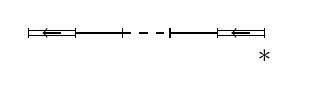
\begin{tikzpicture}[x=.6cm,y=.6cm]
\draw(0,.06)--(1,.06) (0,-.06)--(1,-.06);\draw[->](.7,0)--(.3,0);\draw(1,0)--(2,0);\draw[dashed](2,0)--(3,0);\draw(3,0)--(4,0);\draw(4,.06)--(5,.06) (4,-.06)--(5,-.06);\draw[->](4.7,0)--(4.3,0);\foreach\x in {0,...,5}{\draw(\x,-.1)--(\x,.1);}\node[below]at(5,-.15){$*$};
\end{tikzpicture}\qquad（1）
\end{center}
事实上，容易验证，其余情形 $\Phi_F$ 包含 $G$ 的全部不可倍乘相对根（nonmultipliable relative roots），故断言由 [4，2.23 和 4.3] 得出。在上述例外情形，$\overline G_F^{\mathrm{red}}$ 为特殊正交群，因此不单连通。利用“单连通群中环面的中心化子的导群仍单连通”这一事实，容易得到更一般的结果。称绝对局部 Dynkin 图 $\Delta_1$ 的特殊顶点为好的（good），若它不是该图某个（1）型连通分支的星号顶点。则若 $G$ 半单且单连通，而且 $\bigcup_{v\in I_F}O(v)$ 包含 $\Delta_1$ 每个连通分支中的一个好的特殊顶点，则 $\overline G_F^{\mathrm{red}}$ 的导群单连通。
\origsubsection{3.6}{环面单位群的不动点（Fixed points of groups of units of tori）}
设 $M$ 为 $S$ 的单位群 $S_c=\{s\in S(K)\mid\omega(\chi(s))=0\text{ 对所有 }\chi\in X^*\}$ 的子群。我们要确定：在什么条件下，公寓 $A=A(G,S)$ 恰好等于 $M$ 在 $\mathscr B$ 中的不动点集 $\mathscr B^M$。由 2.2 回顾的建筑性质，$A=\mathscr B^M$，当且仅当对 $A$ 的每个余维一的面 $F$，闭包包含 $F$ 且被 $M$ 固定的室，仅为 $A$ 内具有这些性质的两个室。由 3.5.4，这意味着 $M$ 在 $\overline S(\overline K)$ 中的像 $\overline M$，在 $\overline G_F^{\mathrm{red}}$ 的 $\overline K$ 球面建筑中只有两个不动点。若 $a$ 为 $\Phi_F$ 的两个不可除根之一，这等价于 $a(\overline M)\ne\{1\}$。因此：

\paragraph*{3.6.1.}$A$ 为 $M$ 在 $\mathscr B$ 中完整不动点集的充要条件是，对每个相对根 $a\in\Phi$，有 $a(M)\not\subset1+\mathfrak p$。

特别地，如果 $\overline K$ 至少有四个元素（若 $\overline K\simeq\F_2$），则 $A$ 总是（从不）为 $S_c$ 在 $\mathscr B$ 中的完整不动点集。

前面的讨论还给出如下信息：一个非分裂环面 $S_1$ 在 $K$ 的非分歧 Galois 扩张 $K_1$ 上成为极大分裂环面，则可将 3.6.1 应用于其单位群 $S_{1,c}$ 在 $\mathscr B(G,K_1)$ 上的作用，再利用 2.6.1 作 Galois 下降回到 $\mathscr B$，从而研究 $S_{1,c}$ 的不动点集。例如得到：

若各向异性环面 $S_1$ 在 $K$ 的某个非分歧 Galois 扩张上成为极大分裂环面，则 $S_1(K)$ 在建筑 $\mathscr B$ 中有唯一的不动点。

另一方面，容易证明：若 $S_1$ 是 $G=\SL_2$ 的极大环面，且其分裂域分歧，则 $S_1(K)$ 必固定 $\mathscr B$ 的一个室，也可能固定不止一个室。\footnote{这回答了 G. Lusztig 的一个问题。}对 $\operatorname{PGL}_2$ 中类似的环面 $S_1$，$S_1(K)$ 在 $\mathscr B$ 中可能只有一个不动点，也可能不止一个。
\origsubsection{3.7}{Iwahori 子群；极大紧子群的体积（Iwahori subgroups; volume of maximal compact subgroups）}
本节假设 $G$ 剩余拟分裂；当剩余域 $\overline K$ 有限时，1.10.3保证了这一条件。

为建筑 $\mathscr B$ 的每个室 $C$ 定义一个 $G(K)$ 的子群 $\operatorname{Iw}(C)$，称为对应于 $C$ 的 Iwahori 子群：若 $\overline G_C^\circ$ 为代数群 $\overline G_C$ 的单位分支（见 3.4），则 $\operatorname{Iw}(C)$ 为群 $\overline G_C^\circ(\overline K)$ 在约化同态 $\mathscr G_C(\mathfrak o)\to\overline G_C(\overline K)$ 下于 $\mathscr G_C(\mathfrak o)=G(K)^C$ 中的原像。显然，$G(K)$ 的所有 Iwahori 子群共轭。由 3.5.2，$\overline G_C^\circ$ 可解，故为环面 $\overline T$ 与幺幂群 $\overline U$ 的半直积。由光滑群概形的一般结果，$\operatorname{Iw}(C)$ 是 $\overline T(\overline K)$ 与某个逆极限幂零群（pronilpotent group）$\operatorname{Iw}^u(C)$ 的半直积；若 $\overline K$ 的特征为有限素数 $p$，则 $\operatorname{Iw}^u(C)$ 为pro-$p$ 群（pro-$p$ group）；若 $\overline K$ 有限，$\overline T(\overline K)$ 当然为阶与 $p$ 互素的有限群。

若 $x$ 为 $C$ 的闭包中的一点，则 $\overline G_C^\circ$ 在同态 $\overline\rho_{xC}:\overline G_C\to\overline G_x$ 下的像为 $\overline G_x$ 的一个 Borel 子群 $\overline B$，而 $\overline\rho_{xC}$ 的核是连通幺幂群。因此 $\overline\rho_{xC}$ 将 $\overline G_C^\circ(\overline K)$ 满射到 $\overline B(\overline K)$；再由 3.4.4，$\operatorname{Iw}(C)$ 是 $\overline B(\overline K)$ 在约化同态下于 $G(K)^x=\mathscr G_x(\mathfrak o)$ 中的原像。因此，也可将 $G(K)$ 的 Iwahori 子群定义为：对各 $x\in\mathscr B$，约化群 $\overline G_x$ 的 $\overline K$ Borel 子群在稳定子 $G(K)^x$ 中的原像。

现设 $\overline K$ 有限。则 $G(K)$ 为幺模局部紧群（unimodular locally compact group），Iwahori 子群是紧开子群。因此，存在唯一 Haar 测度 $\mu$，使 Iwahori 子群体积为 $1$。由上，对任意 $x\in\mathscr B$，$G(K)^x$ 关于 $\mu$ 的体积为指数 $[\overline G_x(\overline K):\overline B(\overline K)]$，其中 $\overline B$ 为 $\overline G_x$ 的任一 $\overline K$ Borel 子群。若 $x$ 在包含它的面 $F$ 中处于“一般位置”，则 $\overline G_x=\overline G_F$。已知 $G$ 的局部指标（连同 1.11 的对应 $v\mapsto O(v)$）、$\Delta$ 的顶点集 $I_x$，以及 $\Xi_1=\Xi(G,K_1)$（见 2.5），其中 $K_1$ 为 $K$ 的非分歧闭包，则断言 3.5.2、3.5.3 给出了有效计算这一体积的方法。
\origsubsection{3.8}{超特殊点与子群（Hyperspecial points and subgroups）}
由 3.5.1 与 3.5.3，容易得出 1.10 所定义的 $\mathscr B$ 的超特殊点的如下刻画。

\paragraph*{3.8.1.}$\mathscr B$ 的点 $x$ 超特殊，当且仅当群 $\overline G_x$ 的单位分支约化；此时 $\overline G_x$ 本身连通，因而约化。

还可以证明：$\mathfrak o$ 上一般纤维为 $G$、特殊纤维为约化群的光滑群概形，恰好是超特殊点 $x$ 所对应的概形 $\mathscr G_x$。因此，可将 $G(K)$ 的超特殊子群刻画为这种群概形的单位群。

\paragraph*{3.8.2.}假设 $\overline K$ 有限，且 $G(K)$ 具有超特殊子群（例如，若 $G$ 拟分裂且有非分歧分裂域，此条件成立，见 1.10）；则 $G(K)$ 的超特殊子群，是其全部紧子群中体积最大的那些子群。

利用 3.5 和 3.7，证明并不困难。
\origsubsection{3.9}{整体情形（The global case）}
设 $L$ 为整体域。对 $L$ 的每个有限扩张 $L'$ 及 $L'$ 的每个素位 $v$，以 $\mathfrak o_{L'}$、$\mathfrak o_v$ 分别表示 $L'$ 和其完备化 $L'_v$ 的整数环。设 $H$ 为在 $L$ 上定义的约化线性群。假设将 $H$ 嵌入一般线性群 $\GL_n$，并对上述每组 $L',v$ 定义 $H(\mathfrak o_v)=H(L'_v)\cap\GL_n(\mathfrak o_v)$。也可以通过群概形来描述这个群。考虑由 $L^n$ 中标准格 $\mathfrak o_L^n$ 定义的 $H$ 上的 $\mathfrak o_L$ 群概形结构 $\mathscr H_{\mathfrak o_L}$；更精确地，$\mathscr H_{\mathfrak o_L}$ 是 $H$ 在标准一般线性群概形 $\mathscr{GL}_{n,\mathfrak o_L}$ 中的概形闭包。于是 $H(\mathfrak o_v)=\mathscr H_{\mathfrak o_L}(\mathfrak o_v)$。对包含 $\mathfrak o_L$ 的任一环 $R$，以 $\mathscr H_R$ 表示由 $\mathscr H_{\mathfrak o_L}$ 经基变换所得的 $R$ 上群概形。

\paragraph*{3.9.1.}在 $L$ 的几乎所有有限素位 $v$，$\mathscr H_{\mathfrak o_v}$ 为与建筑 $\mathscr B(H,L_v)$ 的某个超特殊点 $x$ 相联系的群概形 $\mathscr H_x$；因而 $H(\mathfrak o_v)$ 是 $H(L_v)$ 的超特殊子群。

事实上，取 $L$ 的一个使 $H$ 分裂的 Galois 扩张 $L'$，并取一般纤维为 $\mathscr H_{L'}$ 的 $\mathfrak o_{L'}$ 上 Chevalley 群概形 $\mathscr H'_{\mathfrak o_{L'}}$。由于群概形 $\mathscr H_{\mathfrak o_{L'}}$ 与 $\mathscr H'_{\mathfrak o_{L'}}$ 有相同一般纤维，它们在 $L'$ 的几乎所有素位处“相同”。又因 $L'$ 几乎所有素位在其对 $L$ 的限制上非分歧，断言由 3.4.2、3.4.3 及 2.6.1 得到。
\origsubsection{3.10}{例：一般线性群（Example: general linear groups）}
设 $G=\GL_n$。$\GL_n(K)$ 的 Iwahori 子群为与下列子群共轭的子群：\nobreak\footnote{\textbf{译者注（本次校订）：}下式矩阵条件中的最后一个 $i\ge j$ 应为 $i>j$。否则对角元会同时满足 $g_{ii}\in\mathfrak o^\times$ 与 $g_{ii}\in\mathfrak p$，使所定义的集合为空。正确条件为对角元是单位、上三角元属于 $\mathfrak o$、严格下三角元属于 $\mathfrak p$。}
\[
B=\{((g_{ij}))\mid g_{ii}\in\mathfrak o^\times,\ g_{ij}\in\mathfrak o\text{ 若 }i<j,\ g_{ij}\in\mathfrak p\text{ 若 }i\geq j\}.
\]
令 $(b_i)_{1\leq i\leq n}$ 为 $K^n$ 的标准基。对 $1\leq r\leq n$，令 $\Lambda_r$ 为 $K^n$ 中由 $\{b_i/\pi\mid i\leq r\}\cup\{b_i\mid i>r\}$ 生成的格，$P_r$ 为 $\Lambda_r$ 在 $\GL_n(K)$ 中的稳定子。因此，$P_r$ 是全部行列式为单位、且有下列分块形式的矩阵所成的群：
\[
\left(\begin{array}{c|c}
\mathfrak o&\pi^{-1}\mathfrak o\\\hline
\pi\mathfrak o&\mathfrak o
\end{array}\right),\qquad\text{分块大小为 }r\text{ 与 }n-r.
\]
此记号表示，左上角为系数在 $\mathfrak o$ 中的 $r\times r$ 矩阵，右上角为系数在 $\pi^{-1}\mathfrak o$ 中的 $r\times(n-r)$ 矩阵，等等。群 $B$ 是 1.14 所述室 $C$ 在 $\GL_n(K)$ 中的中心化子。子群 $P_r$ 均特殊，每个特殊子群都与其中任一个共轭。各 $P_r$ 是 $\overline C$ 中各一维面上点的稳定子；沿用 2.9 的记号，$P_r$ 固定的点对应于下述形式的范数：
\[
(x_1,\ldots,x_n)\longmapsto\inf\bigl(
\{\omega(x_i)+\omega(\pi)-c\mid i\leq r\}\cup\{\omega(x_i)-c\mid i>r\}\bigr),
\]
其中 $c\in\R$。若 $v$ 为这种点，则概形 $\mathscr G_v$ 是格 $\Lambda_r$ 所定义的“$\GL_n$ 上”的 Chevalley 概形。要描述单位群为 $B$ 的概形 $\mathscr G_C$，可用 $n$ 个标准表示之和将 $\GL_n$ 嵌入 $\GL_{n^2}$，并考虑 $K^{n^2}$ 中的格 $\Lambda_1\oplus\cdots\oplus\Lambda_n$。

注意，$B$ 是 $C$ 中任一点的稳定子。对 $G=\operatorname{PGL}_n$，相应陈述不成立。例如，由 $B$ 与线性变换
\[
b_1\longmapsto b_2\longmapsto\cdots\longmapsto b_n\longmapsto b_1\pi^{-1}\tag{3.10(1)}
\]
生成的群在 $\operatorname{PGL}_n(K)$ 中的像，是投影 $C$ 所得的 $\mathscr B(\operatorname{PGL}_n,K)$ 的室的“重心”$y$ 的稳定子。它也是 $\operatorname{PGL}_n(K)$ 的极大有界子群。概形 $\mathscr G_y$ 可用 $G=\operatorname{PGL}_n$ 的 Lie 代数中的一个格描述，$G$ 通过伴随表示在此 Lie 代数上作用。若 $F$ 为由（1）在 $\operatorname{PGL}_n$ 中的像模 $\mathfrak p$ 约化所生成的 $n$ 阶循环群，则 $\overline G_y$ 是 $F$ 与某个连通群的半直积；特别地，其分支群为 $n$ 阶循环群。
\origsubsection{3.11}{例：奇数维拟分裂特殊酉群（Example: quasi-split special unitary group in odd dimension）}
沿用 1.15 的全部假设与记号，以 $\mathfrak o_L$ 表示 $L$ 的整数环。取 $\lambda\in L$，满足 $\lambda+\lambda^\tau+1=0$、$\omega(\lambda)=\delta$（回顾 $\delta=\sup\{\omega(d)\mid d\in L,d+d^\tau+1=0\}$）。假设一致化元 $\pi_1$ 选得满足 $(\lambda\pi_1)+(\lambda\pi_1)^\tau=0$；$L/K$ 非分歧时这种选择显然可作，分歧时由 1.15（6）得出。

令 $(b_i)_{-n\leq i\leq n}$ 为 $L^{2n+1}$ 的标准基。对 $0\leq r\leq n$，考虑基 $(b_i^{(r)})$：当 $i<-r$ 时 $b_i^{(r)}=b_i/\pi_1$；当 $-r\leq i\leq0$ 时 $b_i^{(r)}=b_i$；当 $i>0$ 时 $b_i^{(r)}=\lambda b_i$。记此基生成的 $\mathfrak o_L$ 格为 $\Lambda_r$。若 $\delta=\omega(\lambda)=0$（除 $L/K$ 分歧且 $\operatorname{char}\overline K=2$ 外总如此），$\Lambda_r$ 也由基 $\{b_i/\pi_1\mid i<-r\}\cup\{b_i\mid i\geq-r\}$ 生成。$\Lambda_r$ 在 $G(K)$ 中的稳定子 $P_r$，也是由下式确定的点 $v_r\in V=A\subset\mathscr B$（按 1.15 的约定）的稳定子：
\[
a_i(v_r)=\begin{cases}\frac12\delta,&i\leq r,\\\frac12(\delta+\omega(\pi_1)),&i>r.\end{cases}
\]
各点 $v_r$ 是由不等式 $\frac12\delta<a_1<\cdots<a_n<\frac12\delta+\frac12\omega(\pi_1)$ 定义的室的顶点。通过 $v\mapsto I_v$，它们按自然的从左到右顺序，对应于 1.15 的图（9）与（10）的顶点。概形 $\mathscr G_{v_r}$ 是由格 $\Lambda_r$ 定义的 $G$ 上的 $\mathfrak o_L$ 结构。

现在简要研究将 $\mathscr G_{v_r}$ 模 $\mathfrak p$ 约化所得的代数群 $\overline G_{v_r}$。固定 $r$，以带撇字母表示关于基 $(b_i^{(r)})$ 的坐标。在这些坐标中，Hermite 型 $h$ 为
\[
\begin{aligned}
h((x'_i),(y'_i))={}&x_0'{}^\tau y'_0+
\sum_{i=1}^r(\lambda^\tau x_i'{}^\tau y'_{-i}+\lambda x_{-i}'{}^\tau y'_i)\\
&+\frac{\lambda^\tau}{\pi_1}\sum_{i=r+1}^n(x_i'{}^\tau y'_{-i}-x_{-i}'{}^\tau y'_i).
\end{aligned}
\]
令 $\widetilde E=\Lambda_r/\pi\Lambda_r$。它是 $\overline K$ 上的 $2(2n+1)$ 维向量空间。可证明自然态射 $\overline G_{v_r}\to\GL(\widetilde E)$ 为单态射（monomorphism）；换言之，$\overline G_{v_r}$ 可视为 $\GL(\widetilde E)$ 的子群。下面分别讨论非分歧与分歧情形。

\paragraph*{第一种情形：L/K 非分歧}此时 $\widetilde E$ 也是 $L$ 的剩余域 $\overline L$ 上的向量空间。反 Hermite 型（antihermitian form）$\pi_1h/\lambda^\tau$ 模 $\pi_1$ 约化为 $\widetilde E$ 上的反 Hermite 型
\[
\overline h_1:((\widetilde x'_i),(\widetilde y'_i))\longmapsto
\sum_{i=r+1}^n(\widetilde x_i'{}^\tau\widetilde y'_{-i}-\widetilde x_{-i}'{}^\tau\widetilde y'_i),
\]
其中横线或波浪号表示相应的约化。令 $\widetilde E_0$ 为此型的核，由 $|i|>r$ 时 $\widetilde x'_i=0$ 定义；令 $\Lambda_{r,0}$ 为 $\widetilde E_0$ 在 $\Lambda_r$ 中的原像。考察 $h$ 在 $\Lambda_{r,0}\times\Lambda_{r,0}$ 上的限制，模 $\mathfrak p$ 约化后成为 $\widetilde E_0$ 上的 Hermite 型
\[
\overline h_2:((\widetilde x'_i)_{-r\leq i\leq r},(\widetilde y'_i)_{-r\leq i\leq r})\longmapsto
\widetilde x_0'{}^\tau\widetilde y'_0+
\sum_{i=1}^r(\overline\lambda^\tau\widetilde x_i'{}^\tau\widetilde y'_{-i}
+\overline\lambda\widetilde x_{-i}'{}^\tau\widetilde y'_i).
\]
最后，$\overline G_{v_r}$ 可描述为型对 $(\overline h_1,\overline h_2)$ 在群 $R_{\overline L/\overline K}(\SL_{\overline L}(\widetilde E))$ 中的稳定子；此群即将 $\overline L$ 向量空间 $\widetilde E$ 的特殊线性群通过标量限制“看作 $\overline K$ 上的代数群”。令 $\widetilde E_1$ 为 $\widetilde E$ 中由 $-r\leq i\leq r$ 时 $\widetilde x'_i=0$ 定义的子空间，以 $\widetilde h_1$ 表示 $\overline h_1$ 在 $\widetilde E_1\times\widetilde E_1$ 上的限制。则 $\overline G_{v_r}$ 显然包含群 $\operatorname{SU}(\widetilde h_1)\times\operatorname{SU}(\overline h_2)$，它正是其 Levi 子群 $\overline G_{v_r}^{\mathrm{red}}$（见 3.5）。\footnote{\textbf{译者注（本次校订）：}当两个非退化块均非零时，这里列出的 $\operatorname{SU}(\widetilde h_1)\times\operatorname{SU}(\overline h_2)$ 是 Levi 子群的导出群；完整的 Levi 子群为 $\operatorname{S}(\operatorname U(\widetilde h_1)\times\operatorname U(\overline h_2))$，即两块酉变换的行列式乘积为一的群。两块的行列式不必分别为一，因此还有一个一维中心环面。}注意，符合 3.5.1，从 1.15 的图（9）删去第 $(r+1)$ 个顶点及邻接边所得图为 $BC_r\times C_{n-r}$ 型，这确实为 $\operatorname{SU}(\widetilde h_1)\times\operatorname{SU}(\overline h_2)$ 的相对根系类型。

\paragraph*{第二种情形：L/K 分歧}此时，$\Lambda_r$ 中的标量乘法 $\pi_1$，模 $\pi$ 约化后给出自同态 $\nu:\widetilde E\to\widetilde E$，它显然被 $\overline G_{v_r}$ 中心化，且核等于像 $\nu(\widetilde E)$。商 $\overline E=\widetilde E/\nu(\widetilde E)$ 典范同构于 $\Lambda_r/\pi_1\Lambda_r$，将二者等同。$\nu$ 被 $\overline G_{v_r}$ 中心化，故投影 $\widetilde E\to\overline E$ 诱导 $\overline K$ 代数群同态 $\overline G_{v_r}\to\GL(\overline E)$，其核幺幂。这里只描述此同态的像，记作 $\overline G'_{v_r}$；确定 $\overline G_{v_r}$ 的完整结构留作练习。

将反 Hermite 型 $\pi_1h/\lambda^\tau$ 模 $\pi_1$ 约化，得到 $\overline E$ 上的交错型（alternating form）
\[
\overline h_1:((\overline x'_i),(\overline y'_i))\longmapsto
\sum_{i=r+1}^n(\overline x'_i\overline y'_{-i}-\overline x'_{-i}\overline y'_i).
\]
令 $\overline E_0$ 为此型的核，由 $|i|>r$ 时 $\overline x'_i=0$ 定义；$\Lambda_{r,0}$ 为其在 $\Lambda_r$ 中的原像。现考察 $q:\Lambda_{r,0}\to K$，$q(x)=h(x,x)$。经约化后，它成为二次型 $\overline q:\overline E_0\to\overline K$：
\[
\overline q((\overline x'_i)_{-r\leq i\leq r})=\overline x_0'{}^2-
\sum_{i=1}^r\overline x'_{-i}\overline x'_i.
\]
最后，$\overline G'_{v_r}$ 是 $\SL(\overline E)$ 中保持 $\overline h_1$、且在 $\overline E_0$ 上诱导（既约）群 $\operatorname{SO}(\overline q)$ 的一个元素的全部元素组成的群。令 $\overline E_1$ 为由 $-r<i<r$ 时 $\overline x'_i=0$ 定义的 $\overline E$ 的子空间，以 $\widetilde h_1$ 表示 $\overline h_1$ 在 $\overline E_1\times\overline E_1$ 上的限制。\footnote{\textbf{译者注（本次校订）：}此处定义 $\overline E_1$ 时，坐标范围应为 $-r\le i\le r$，即应令这些坐标全部为零。使用严格不等式会留下核中的端点坐标（$r=0$ 时也会留下零坐标），使 $\widetilde h_1$ 退化，不能得到所写的辛群。}则 $\operatorname{Sp}(\widetilde h_1)\times\operatorname{SO}(\overline q)$ 是 $\overline G'_{v_r}$ 的 Levi 子群，它是 $\overline G_{v_r}$ 的 Levi 子群 $\overline G_{v_r}^{\mathrm{red}}$ 在该群中的同构像。如非分歧情形一样，可检验 3.5.1；此时使用 1.15 的图（10），得到 $\overline G_{v_r}^{\mathrm{red}}$ 的根系类型 $B_r\times C_{n-r}$。

注意，即使在非分歧情形，也可不用 $h$ 在 $\Lambda_{r,0}\times\Lambda_{r,0}$ 上的限制，而考察其“收缩”$q:\Lambda_{r,0}\to K$、$q(x)=h(x,x)$，这样，两种情形便可采用更统一的处理方式。另一方面，引入 $\lambda$ 是为尽量减少情形划分；在非分歧情形，以及 $\operatorname{char}\overline K\ne2$ 时，可以到处以 $1$ 代替 $\lambda$，使方程有所简化。
\origsubsection{3.12}{例：拟分裂但不分裂的特殊正交群（Example: quasi-split but nonsplit special orthogonal group）}
现采用 1.16 的假设与记号，只是取 $G$ 为特殊正交群 $\operatorname{SO}(q)$。这里只讨论这一例子的一个方面：构造建筑的一个顶点 $v$，使 $\overline G_v$ 不连通。假设 $L/K$ 非分歧。令 $\Lambda$ 为 $K^n\oplus L\oplus K^n$ 中的格 $\mathfrak o^n\oplus\pi\mathfrak o_L\oplus\mathfrak o^n$，其中 $\mathfrak o_L$ 为 $L$ 的整数环。$\Lambda$ 在 $G(K)$ 中的稳定子 $P$，也是由 $a_i(v)=\frac12\omega(\pi)$（$1\leq i\leq n$）定义的点 $v\in V\subset A$ 的稳定子；它是 1.16 所描述的室的一个顶点。在 1.16 的图（1）中，$I_v$ 为最左端的顶点。如 3.11，可将 $\overline G_v$ 描述为 $\GL(\widetilde E)$ 的子群，其中 $\widetilde E=\Lambda/\pi\Lambda$ 为 $\overline K$ 向量空间。型 $q$ 在 $\Lambda$ 上的限制经约化，成为 $\widetilde E$ 上的二次型 $\widetilde q:(\widetilde x_i)_{-n\leq i\leq n}\mapsto\sum_{i=1}^n\widetilde x_{-i}\widetilde x_i$，其中横线或波浪号表示相应的约化（$i=0$ 时 $\widetilde x_i$ 属于 $L$ 的剩余域，否则属于 $\overline K$）。令 $\widetilde E_0$ 为 $\widetilde q$ 的二维核，由 $i\ne0$ 时 $\widetilde x_i=0$ 定义；令 $\overline q$ 为 $\widetilde q$ 在 $\overline E=\widetilde E/\widetilde E_0$ 上诱导的二次型。显然，$\overline G_v$ 保持型 $\widetilde q$。因此投影 $\widetilde E\to\overline E$ 诱导 $\overline K$ 同态 $\overline G_v\to O(\overline q)$。可验证，此同态满射（特别地，$\overline G_v$ 不连通），并将 $\overline G_v^{\mathrm{red}}$ 同构地映到 $\operatorname{SO}(\overline q)$。\footnote{\textbf{译者注（本次校订）：}这个映射在 Levi 子群上还有一个各向异性的一维环面核。原二次型的 $L$ 分量上的范数一变换保留格 $\Lambda$，经约化后仍在二维核 $\widetilde E_0$ 上非平凡作用，却在 $\overline E$ 上作用平凡。因此完整的连通 Levi 子群为 $\operatorname{SO}(\overline q)\times\operatorname{SO}(N_{\overline L/\overline K})$；到第一因子的投影不能称为同构。}若 $\tau$ 为 $L$ 的非平凡 $K$ 自同构，则属于 $P$ 的线性变换
\[
(x_i)_{-n\leq i\leq n}\longmapsto(x_n,x_{-n+1},\ldots,x_{-1},x_0^\tau,x_1,\ldots,x_{n-1},x_{-n})
\]
经约化给出 $\overline G_v(\overline K)$ 的一个元素，它映入 $O(\overline q)$，但不映入 $\operatorname{SO}(\overline q)$。
